\section{Preparación del entorno de trabajo}

Como decía Robert Owen, un reconocido empresario galés, en el siglo XVIII:

\begin{displayquote}
    Mejorando el entorno se mejora al hombre.
\end{displayquote}

El desarrollo de esta preparación previa ha supuesto un ahorro de tiempo bastante grande para el proyecto.
\\Esta sección irá estructurada en consonancia a la cronología de creación de cada parte del entorno. Empezando por la semilla de todo: Github.

\subsection{GitHub}
El proyecto se realizará en GitHub. Esto se hace de forma muy rápida y fácil.

\begin{enumerate}
    \item Hay que dirigirse a la dirección de \url{github.com}. Donde podrá observarse algo parecido a la figura \ref{pagina_principal_github}.
          \begin{figure}[htbp]
              \centering
              
\includegraphics[scale=0.3]{preparacion_entorno/pagina_principal_github.png}
              \caption{Página principal de GitHub}\label{pagina_principal_github}
          \end{figure}
    \item En la parte superior derecha aparecerá ``Sign up'' donde se clicará para poder registrarse dentro de la web.
    \item Una vez se haya realizado el registro se volverá a \url{github.com} y se clicará a la izquierda de ``Sign up'' que pone ``Sign in'' donde podrá iniciarse sesión.
    \item Cuando se haya iniciado sesión hay que dirigirse a la parte superior izquierda clicando en ``new'' para crear un nuevo repositorio.
    \item Se rellenarán los campos que se solicitan para crear un nuevo repositorio. Se le dará el nombre de Inventarium al repositorio y se marcará en la casilla para que sea privado. También se procederá a añadirle un archivo del tipo Readme para poder describir partes del proyecto dentro de este. Por último se pulsará sobre el botón ``Create repository'' como puede verse en la figura \ref{creando_repositorio_github}.
          \begin{figure}[htbp]
              \centering
              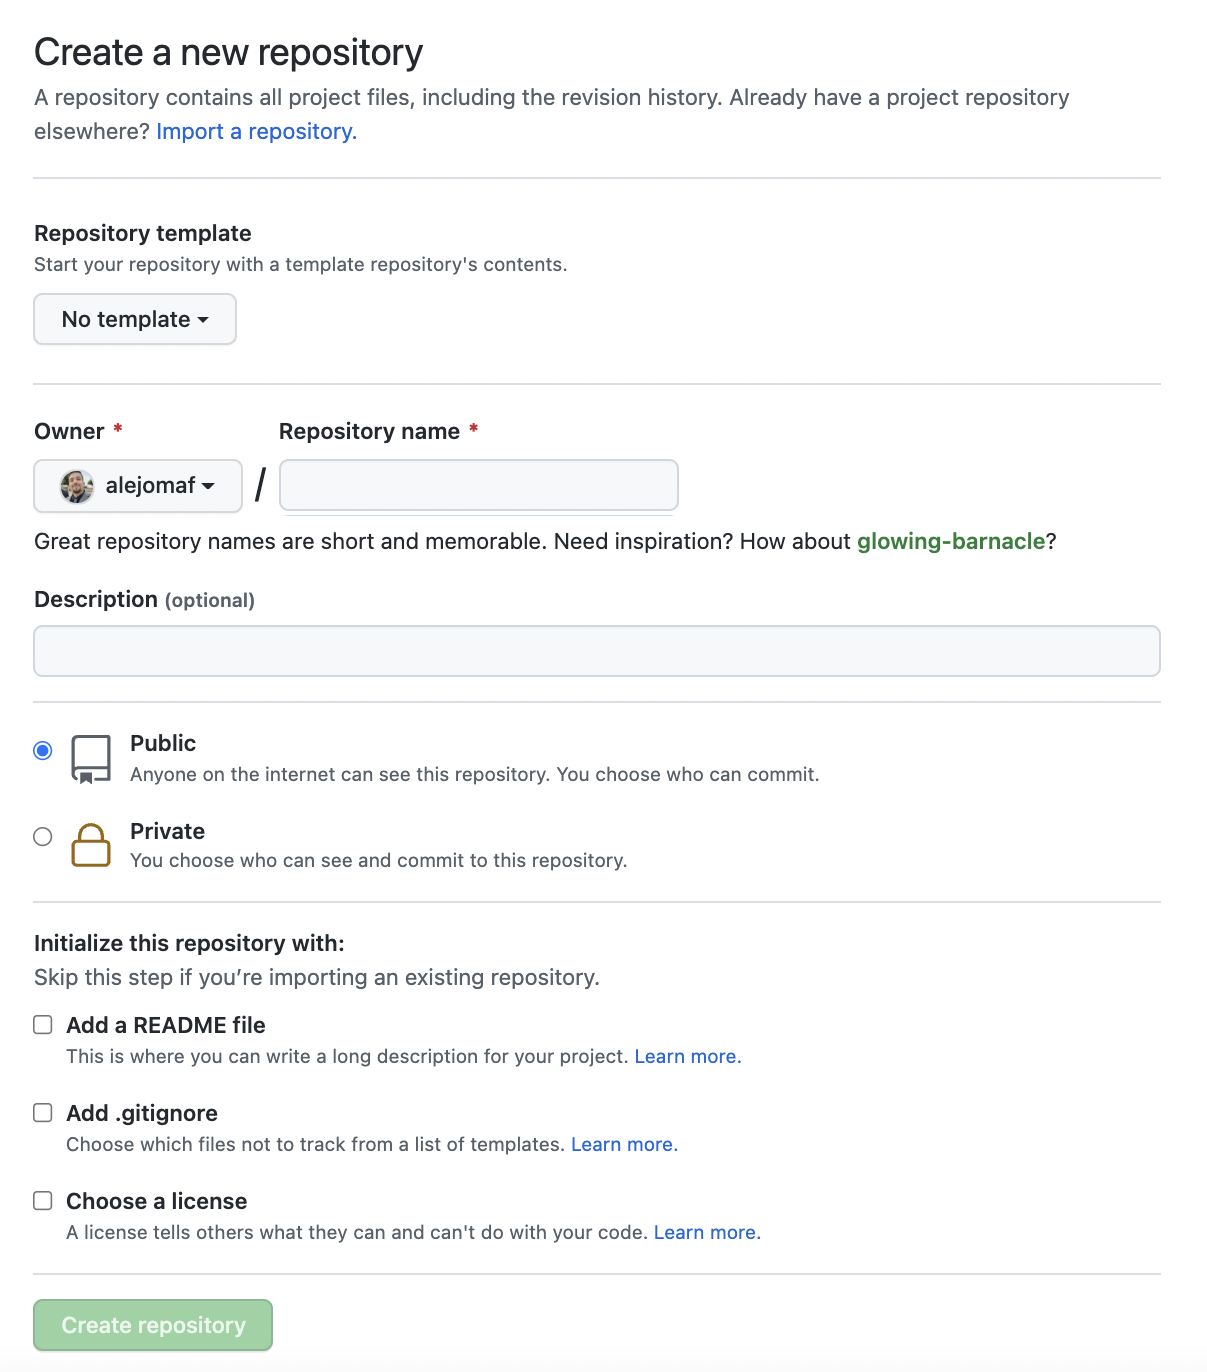
\includegraphics[scale=0.4]{preparacion_entorno/creando_nuevo_repositorio.png}
              \caption{Creando un nuevo repositorio dentro de GitHub}\label{creando_repositorio_github}
          \end{figure}
\end{enumerate}

Con estos sencillos pasos se ha realizado la creación del repositorio del proyecto.

\subsection{Visual Studio Code y Google Cloud, los mejores amigos}
Hoy en día lo nuevo y a lo que la sociedad se dirige es la nube. Dentro de ella se pretenden que se realicen todos los procesos. La mayoría de herramientas y servicios que se nos ofrece cumplen un modelo de caja negra. Es decir, se puede interactuar con ellos y recibir respuestas pero no puede verse qué procesos ocurren dentro de aquella caja.
\\Por esta razón cada vez se empieza a disponer menos de un software como tal y se empiezan a pasar a servicios en línea. Esto no quiere decir que se dejen de usar programas o aplicaciones móviles. Pero la realidad es que sin internet; la mayoría no funcionaría.
\\Esto presenta desventajas siendo la principal que se depende constantemente de una conexión en línea que puede parecer que está presente en todos sitios pero en lugares remotos de la ciudad, como son los pueblos de montaña, el internet no es el mejor compañero, por decirlo, de una manera.
\\Las ventajas son enormes aunque solo se verán las que implican mayor relevancia para el desarrollo del proyecto.
\\El tener ya un repositorio generado con el proyecto subido dentro de él aporta bastante autonomía ya que puede accederse a él y descargar los datos desde cualquier lugar. Pero, ¿y configurarlo?
\\Aquí viene una problemática que no resuelve un entorno de repositorios. El tener que configurarlo todo cada vez que se quiera trabajar desde un sitio distinto. Esto lo resuelven las máquinas virtuales en la nube. El generar un directorio de trabajo donde poder conectar el Visual Studio Code y olvidarse de preocupaciones.
\\Lo segundo que se ha considerado más importante es el ahorro de memoria tanto de RAM como de disco y de procesos que se origina al hacer esto. No es lo mismo tener que trabajar con un portátil conectado todo el día a un enchufe que poder ir llevándolo contigo durante todo el día por el escaso consumo de batería que tiene. Peor si es una torre, solo puedes trabajar desde un único sitio, con la problemática también de que siempre se te puede ir la luz.
\\Estas ventajas expuesta son las que favorecen al desarrollo del proyecto que es realizado por una única persona, pero ¿y si este se hiciera en un equipo? El poder tener varias personas trabajando en el mismo proyecto, tocando los distintos componentes que se están desarrollando dentro de la aplicación es fantástico.

\subsubsection{Crear una máquina virtual en Google Cloud}
Los pasos para la creación de una máquina virtual son:

\begin{enumerate}
    \item El registro es fácil de realizar ya que la herramienta es propiedad de Google. Se omitirá este paso.
    \item Google Cloud se organiza mediante proyectos. Esto brinda facilidades a la hora de calcular el gasto que se tendrá por el uso de la computación en la nube. Aparte de poder facilitar la búsqueda por cada proyecto que se tenga activo. Se procederá a crear un nuevo proyecto clicando arriba a la izquierda a la derecha del título de la página y posteriormente clicando en nuevo proyecto.
    \item Luego se desplegará la barra lateral de la izquierda y se clicará en el apartado de Compute Engine.
    \item Se pulsará el botón de crear instancia. A la hora de rellenar los parámetros se ha comprobado que no es necesario darle demasiada importancia a la zona o región donde se ubique tu máquina. Esta se conectará con una velocidad bastante decente. En el apartado de configuración de máquina con 2GB de RAM y 1VCPU se tendrán suficientes recursos. El tamaño del disco eligido será de 20GB. Dentro de la sección Firewall se habilitará el tráfico HTTP y HTTPS. Y posteriormente se pulsará en crear.
    \item Después de haber creado la máquina se le asignará una IP estática pública que se usará para conectarse a ella mediante SSH.
    \item En el momento de haber creado la máquina esta ha dado una clave privada SSH para poder conectarse a ella. Es necesario guardarla.
\end{enumerate}

\subsubsection{Configurar claves SSH}

Teniendo ya la clave privada SSH de la máquina virtual se utilizará para realizar la conexión con ella. Pero para ello es necesario configurarla. Hay que acceder al fichero usuario/.ssh/config y añadir tres nuevas líneas:
\begin{verbatim}
    Host "Dirección IP"
    HostName "Nombre del host"
    User "Nombre de usuario"
\end{verbatim}
Lo último que nos queda es realizar la conexión mediante SSH a la máquina con Visual Studio Code.

\subsubsection{Realizar conexión SSH mediante Visual Studio Code}
Dentro del apartado de extensiones de Visual Studio Code se localizarán los siguientes plugins para instalar:

\begin{itemize}
    \item Remote - SSH
    \item Remote - SSH: Editing Configuration Files
\end{itemize}

Luego de la instalación de estas dos extensiones se procederá a realizar la conexión. Abajo a la izquierda aparecerá la opción de poder conectarse mediante SSH. Hay que clicar sobre ella y luego se pulsará en ``Connect to Host'' añadiendo la dirección IP estática pública que dio Google Cloud.
\\Ya con esto estaría la masa del entorno hecha, solo hace falta darle un poco de forma y calor para poder finalizarla.

\subsection{Instalación de las extensiones de Visual Studio Code dentro de la MV}

Esta es la lista de componentes con la que se trabajará en todas las fases del proyecto. Hay que acceder a las extensiones dentro de Visual Studio Code y proceder a instalarlas dentro de la máquina virtual.

\begin{itemize}
    \item Docker
    \item LaTeX
    \item LaTeX Workshop
\end{itemize}

Los complementos de Latex ayudarán más tarde con la redacción del Trabajo de Fin de Grado.
\\En Visual Studio Code también se instalará:

\begin{itemize}
    \item Bootstrap 4 snippets
    \item HTML snippets
    \item CSS snippets
\end{itemize}

\subsection{Configuración de la máquina virtual}

Desde Visual Studio Code se accederá a la terminal de la máquina virtual. Se pinchará en ``Ver'' en la sección superior y luego en Terminal. Desde ahí se podrá controlar la máquina.

\subsubsection{Actualización del sistema}
Se realizará una actualización del sistema para evitar posibles fallos en un futuro:
\begin{verbatim}
    sudo apt-get update
    sudo apt-get upgrade
\end{verbatim}

\subsubsection{Instalación de Node JS}
\begin{verbatim}
    sudo apt install nodejs
\end{verbatim}

\subsubsection{Instalación de Angular 12}
\begin{verbatim}
    sudo npm install npm@latest -g
    sudo npm install -g @angular/cli
\end{verbatim}

\subsubsection{Instalación de Docker y Docker Compose}
\begin{verbatim}
    \\Instalacion de Docker

    sudo apt install apt-transport-https ca-certificates
    curl software-properties-common
    curl -fsSL https://download.docker.com/linux/ubuntu/gpg
    sudo apt-key add -
    sudo add-apt-repository 
    "deb [arch=amd64] https://download.docker.com/linux/ubuntu focal stable"
    sudo apt install docker-ce

    \\Instalacion de Docker Compose

    sudo curl -L "https://github.com/docker/compose/releases/download/1.26.0
    /docker-compose-$(uname -s)-$(uname -m)" -o /usr/local/bin/docker-compose
    sudo chmod +x /usr/local/bin/docker-compose
\end{verbatim}

\subsubsection{Configuración de credenciales de Git e instalación del repositorio}
\begin{verbatim}
    //Configuración de credenciales

    git config --global user.name "tu nombre de usuario"
    git config --global user.email "tu correo electrónico"
    git config --global user.password "tu contraseña"

    //El repositorio se ubicará dentro de la carpeta raíz del usuario
    
    git clone https://github.com/alejomaf/Inventarium.git
\end{verbatim}